\documentclass{beamer}

\mode<presentation> {

% The Beamer class comes with a number of default slide themes
% which change the colors and layouts of slides. Below this is a list
% of all the themes, uncomment each in turn to see what they look like.

%\usetheme{default}
%\usetheme{AnnArbor}
%\usetheme{Antibes}
%\usetheme{Bergen}
%\usetheme{Berkeley}
%\usetheme{Berlin}
%\usetheme{Boadilla}
%\usetheme{CambridgeUS}
%\usetheme{Copenhagen}
%\usetheme{Darmstadt}
%\usetheme{Dresden}
\usetheme{Frankfurt}
%\usetheme{Goettingen}
%\usetheme{Hannover}
%\usetheme{Ilmenau}
%\usetheme{JuanLesPins}
%\usetheme{Luebeck}
%\usetheme{Madrid}
%\usetheme{Malmoe}
%\usetheme{Marburg}
%\usetheme{Montpellier}
%\usetheme{PaloAlto}
%\usetheme{Pittsburgh}
%\usetheme{Rochester}
%\usetheme{Singapore}
%\usetheme{Szeged}
%\usetheme{Warsaw}

% As well as themes, the Beamer class has a number of color themes
% for any slide theme. Uncomment each of these in turn to see how it
% changes the colors of your current slide theme.

%\usecolortheme{albatross}
%\usecolortheme{beaver}
%\usecolortheme{beetle}
\usecolortheme{crane}
%\usecolortheme{dolphin}
%\usecolortheme{dove}
%\usecolortheme{fly}
%\usecolortheme{lily}
%\usecolortheme{orchid}
%\usecolortheme{rose}
%\usecolortheme{seagull}
%\usecolortheme{seahorse}
%\usecolortheme{whale}
%\usecolortheme{wolverine}

%\setbeamertemplate{footline} % To remove the footer line in all slides uncomment this line
%\setbeamertemplate{footline}[page number] % To replace the footer line in all slides with a simple slide count uncomment this line

%\setbeamertemplate{navigation symbols}{} % To remove the navigation symbols from the bottom of all slides uncomment this line
}

\usepackage{extpfeil}
\usepackage{extarrows} %Allows long equation signs
\usepackage{graphicx} % Allows including images
\usepackage{booktabs} % Allows the use of \toprule, \midrule and \bottomrule in tables
\usepackage{physics}
\usepackage{tikz}
\usepackage{cite}

%花体字母
\usepackage{amsthm,amsmath,amssymb}
\usepackage{mathrsfs}
\usepackage{dutchcal}

\definecolor{tianyiblue}{rgb}{135,206,250}
%----------------------------------------------------------------------------------------
%	TITLE PAGE
%----------------------------------------------------------------------------------------

\title[VP260 RC]{VP260 Recitation Class 1} % The short title appears at the bottom of every slide, the full title is only on the title page

\author{Yanjun Chen} % Your name
\institute[UM-SJTU JI] % Your institution as it will appear on the bottom of every slide, may be shorthand to save space
{
    University of Michigan - Shanghai Jiao Tong University Joint Institute\\% Your institution for the title page
\medskip
}
\date{\today} % Date, can be changed to a custom date

\begin{document}

\begin{frame}
    \titlepage % Print the title page as the first slide
\end{frame}





\section{Vector Calculus} % Section title slide, unnumbered


\begin{frame}{Vector Algebra}	
	\begin{itemize}
		\item vector addition: $\va{v} + \va{u} $
		\item scalar multiplication: $\lambda \va{v}$
		\item dot product: $\va{v} \vdot \va{u}$
		\item cross product: $\va{v} \cp \va{u}$
		\item scalar triple product: $\va{a} \vdot (\va{b} \cp \va{c}) =\va{b} \vdot (\va{c} \cp \va{a}) = \va{c} \vdot (\va{a} \cp \va{b})$
		\item vector triple product: $\va{a} \cp (\va{b} \cp \va{c}) = \va{b} (\va{a} \cdot \va{c}) - \va{c} (\va{a} \cdot \va{b})$
	\end{itemize}
\end{frame}

\begin{frame}{Differential Calculus}
	\begin{itemize}
		\item gradient: $$\grad f = \pdv{f}{x} \vu{x} + \pdv{f}{y} \vu{y} + \pdv{f}{z} \vu{z}$$
		\item divergence: $\div{\va{v}}$
		\item curl: $$\curl{\va{v}} = \vu{x} \left(\pdv{v_z}{y} - \pdv{v_y}{z}\right) + \vu{y} \left( \pdv{v_x}{z} - \pdv{v_z}{x}\right) + \vu{z} \left( \pdv{v_y}{x} - \pdv{v_x}{y}\right)$$
	\end{itemize}	
\end{frame}

\begin{frame}{Stoke's formula}
	\begin{beamerboxesrounded}{Foundamental theorem for gradients}
		\begin{equation}
			\int_{\vb{a}}^{\vb{b}} (\grad f) \vdot \dd{\vb*{l}} = f(\vb{b}) - f(\vb{a})
		\end{equation}
	\end{beamerboxesrounded}
	
	\begin{beamerboxesrounded}{Divergence theorem}
		\begin{equation}
			\int_V (\div \vb{v}) \dd{\tau} = \oint_{\partial V} \vb{v} \vdot \dd{\vb*{A}}
		\end{equation}
	\end{beamerboxesrounded}

	\begin{beamerboxesrounded}{Stoke's theorem}
		\begin{equation}
			\int_S (\curl \vb{v}) \vdot \dd{\vb{A}} = \oint_{\partial S} \vb{v} \vdot \dd{\vb{l}}
		\end{equation}
	\end{beamerboxesrounded}
\end{frame}





\section{Electrostatics}

\begin{frame}{Charges and Laser Printing}
	\begin{itemize}
		\item positive(+), negative(-)
		\item electric charge: $Q$ (unit: [C])
		\item charges with different signs attract each other
	\end{itemize}
	\vspace{.5em}
	\begin{figure}[htbp]
		\centering
		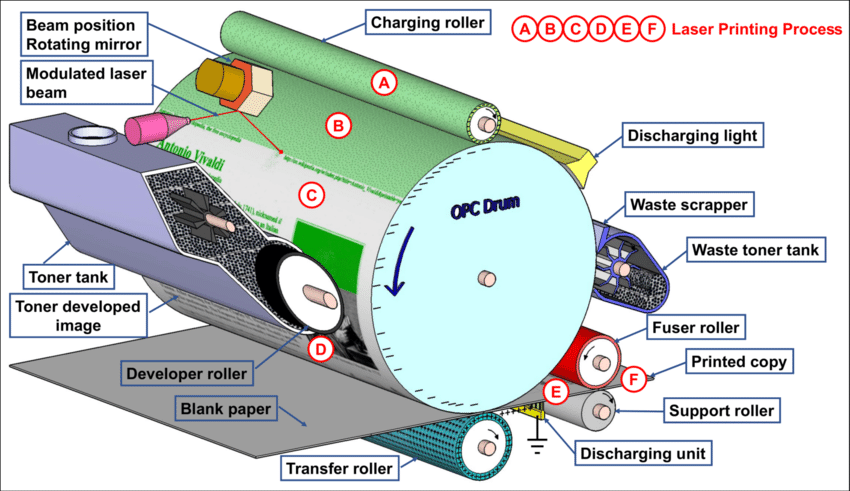
\includegraphics[width=8cm]{Images/Laser-printer}
		\caption{Laser Printing}
	\end{figure}
\end{frame}

\begin{frame}{Coulomb Force}	
	\begin{beamerboxesrounded}{Coulomb Force}
		\begin{equation}
			\vec{F} = \frac{1}{4\pi\epsilon_0} \frac{\abs{q_1 q_2}}{r^2} \vu{r}
		\end{equation}	
    \end{beamerboxesrounded}

	\begin{itemize}
		\item permittivity of vacuum: $\epsilon_0 = 8.85 \times 10^{-12} \  C^2/(N \cdot m^2)$
		\item The direction of $\vu{r}$ is decided by charges.
	\end{itemize}
\end{frame}

\begin{frame}{Superposition Principle}
	\begin{columns}
		\begin{column}{.5\textwidth}
			\begin{figure}[htbp]
				\centering
				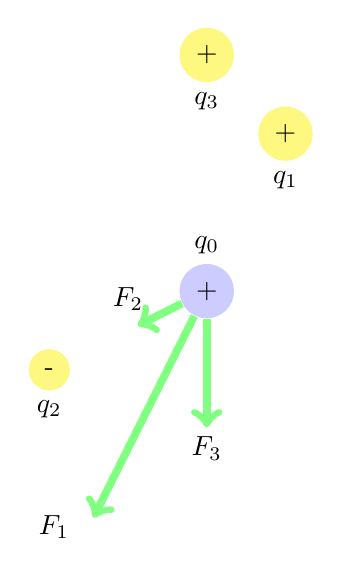
\begin{tikzpicture}
					\node[fill=blue!20, circle, label=above:$q_0$] (X0) at (5,5) {+};
					\node[fill=yellow!50, circle, label=below:$q_1$] (X1) at (6,7) {+};
					\node[fill=yellow!50, circle, label=below:$q_2$] (X2) at (3,4) {-};
					\node[fill=yellow!50, circle, label=below:$q_3$] (X3) at (5,8) {+};
					\node[] (X3') at (5,3) {$F_3$};
					\node[label=above:$F_2$] (X2') at (4,4.5) {};
					\node[label=left:$F_1$] (X1') at (3.5,2) {};
					\draw[-to, line width=.1cm, green!50] (X0) -- (X3');
					\draw[-to, line width=.1cm, green!50] (X0) -- (X2');
					\draw[-to, line width=.1cm, green!50] (X0) -- (X1');
				\end{tikzpicture}
			\end{figure}
			
		\end{column}

		\begin{column}{.5\textwidth}
			\begin{equation}
				\va{F} = \va{F_1} + \va{F_2} + \va{F_3}
			\end{equation}
		\end{column}
	\end{columns}
\end{frame}


\begin{frame}{Electric Field}	
	\begin{beamerboxesrounded}[shadow=true]{\bf Electric Field}
        \begin{equation}
			\vec{E} = \frac{\vec{F}}{q_0}
		\end{equation}
    \end{beamerboxesrounded}
	
	\begin{itemize}
		\item Only valid when $q_0$ is a point charge.
		\item Electric field is a vector field in space.
		\item "real" physical entity
		\item unit: $V/m$ or $N/C$
	\end{itemize}
\end{frame}

\begin{frame}{Electric Field Lines}
	\begin{figure}[htbp]
		\centering
		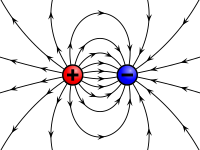
\includegraphics[width=0.3\textwidth]{Images/ele_field.png}
		\caption{Electrical field}
	\end{figure}

	\begin{itemize}
		\item $\va{E}$ is tangential to the field line.
		\item Field lines only intersect at point charges.
		\item Density of field line represents the magnitude of $\va{E}$.
	\end{itemize}
\end{frame}

\begin{frame}{Superposition Principle}
	\begin{columns}
		\begin{column}{.5\textwidth}
			\begin{figure}[htbp]
				\centering
				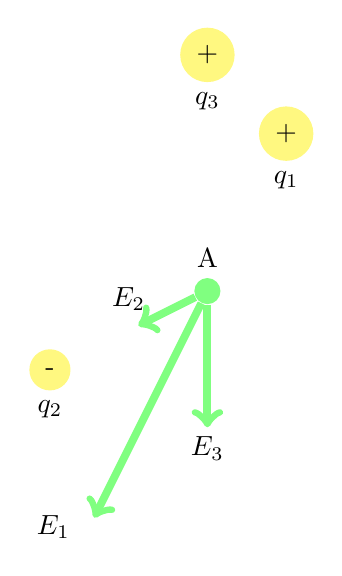
\begin{tikzpicture}
					\node[fill=green!50, circle, label=above:A] (X0) at (5,5) {};
					\node[fill=yellow!50, circle, label=below:$q_1$] (X1) at (6,7) {+};
					\node[fill=yellow!50, circle, label=below:$q_2$] (X2) at (3,4) {-};
					\node[fill=yellow!50, circle, label=below:$q_3$] (X3) at (5,8) {+};
					\node[] (X3') at (5,3) {$E_3$};
					\node[label=above:$E_2$] (X2') at (4,4.5) {};
					\node[label=left:$E_1$] (X1') at (3.5,2) {};
					\draw[-to, line width=.1cm, green!50] (X0) -- (X3');
					\draw[-to, line width=.1cm, green!50] (X0) -- (X2');
					\draw[-to, line width=.1cm, green!50] (X0) -- (X1');
				\end{tikzpicture}
			\end{figure}
			
		\end{column}

		\begin{column}{.5\textwidth}
			\begin{equation}
				\va{E} = \va{E_1} + \va{E_2} + \va{E_3}
			\end{equation}

			If we put a point charge $q_0$ at A, the Coulomb force will be,
			\begin{equation}
				\va{F} = q_0 \va{E}.
			\end{equation}
		\end{column}
	\end{columns}
\end{frame}

\begin{frame}{Continuous Charge Distributions}
	\begin{beamerboxesrounded}{Charge density}
		$\rho(\va{r}) : \mathbb{R}^3 \to \mathbb{R}$ [$C/m^3$]
	\end{beamerboxesrounded}

	\begin{itemize}
		\item The electric charge in a particular volume $V$ is,
		\begin{equation}
			Q = \int_V \rho(\vb{r}) \dd{\tau}.
		\end{equation}

		\item We can define line charge density $\lambda(\vb{r})$ and surface charge density $\sigma(\vb{r})$ similarly.
	\end{itemize}

	\begin{beamerboxesrounded}{Electronic field for continuous distribution}
		\begin{equation}
			\va{E} (\va{r}) = \frac{1}{4 \pi \epsilon_0 } \int \frac{\rho(\va{r'})}{\abs{\mathbcal{r}}^2} \vu{\mathbcal{r}} \dd{\tau} 
		\end{equation}
		
	\end{beamerboxesrounded}
	\begin{itemize}
		\item $\va{\mathbcal{r}} = \va{r'} - \va{r}$
	\end{itemize}
\end{frame}

\begin{frame}{Dirac delta}
	\textbf{How to consider point charge as a "continuous" distribution?}
	\begin{itemize}
		\item It should be infinity at a point and zero elsewhere.
	\end{itemize}

	\begin{beamerboxesrounded}{Dirac delta}
		\begin{equation}
			\delta(x) = \begin{cases}
						\infty, & x = 0\\
						0,& x \neq 0
						\end{cases}
		\end{equation}
	\end{beamerboxesrounded}

	\begin{itemize}
		\item It is not a function!
		\item We can define it in mathematics as "generalized functions" or "distributions".
		\item important property: $$\int \delta(x - a) f(x) \dd{x} = f(a) $$
	\end{itemize}
\end{frame}

\begin{frame}{Electric Dipole}
	\begin{figure}[htbp]
		\centering
        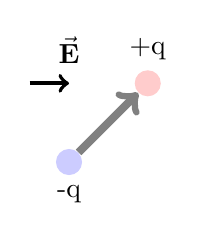
\begin{tikzpicture}
			\node[fill=blue!20, circle, label=below:-q] (N) at (0,0) {};
			\node[fill=red!20, circle, label=above:+q] (P) at (1,1) {};
			\draw[-to, line width=.1cm, black!50] (N) -- (P);
			\draw[-to, line width=.05cm, black] (-0.5,1) -- (0,1);
			\node[label=above:$\va{E}$] (E) at (0,1) {};
		\end{tikzpicture}
	\end{figure}

	\begin{beamerboxesrounded}{Electric dipole}
        \begin{equation}
			\va{p} = q \va{l}
		\end{equation}
		\begin{equation}
			\va{\tau} = \va{p} \cp \va{E}
		\end{equation}
		\begin{equation}
			U = - \va{p} \vdot \va{E}
		\end{equation}
    \end{beamerboxesrounded}
\end{frame}

\begin{frame}{Gauss' Law}
	\begin{beamerboxesrounded}{Electric flux}
		\begin{equation}
			\Phi_E = \int_{S} \va{E} \vdot \dd{\va{A}}
		\end{equation}
	\end{beamerboxesrounded}
	\vspace{1em}
	\begin{beamerboxesrounded}{Gauss' law}
		\begin{equation}
			\oint_{S} \va{E} \cdot \dd{\va{A}} = \frac{q_{enc}}{\epsilon_0}
		\end{equation}
		\begin{equation}
			\div \va{E} = \frac{\rho(\vec{r})}{\epsilon_0}
		\end{equation}
	\end{beamerboxesrounded}
	\begin{itemize}
		\item The $q_{enc}$ is the total charge enclosed in the surface.
	\end{itemize}
\end{frame}








\section{Exercise}

\begin{frame}{Exercise 1}
	Find the electric field a distance $z$ above the center of a square loop (side $a$) carrying uniform line charge $\lambda$.
	\begin{figure}[htbp]
		\centering
		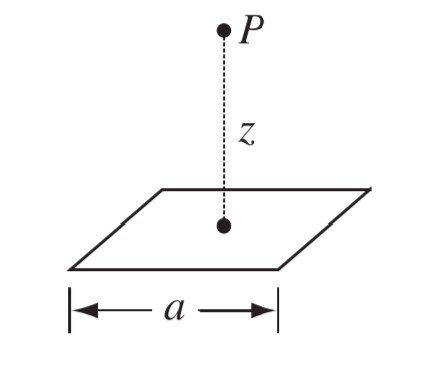
\includegraphics{Images/ex1.jpg}
	\end{figure}
\end{frame}

\begin{frame}{Exercise 2}

An infinite cylinder of radius R is charged non-uniformly
with the density of charge $\rho=Ar$, where A is a positive
constant. Find the electric field at any point of space.
(consider both: $r<R$ and $r>R$)

\end{frame}

\begin{frame}{Exercise 3}
	Consider a uniform insulating ball with bulk density of charge $\rho < 0$. Imagine that a part of the ball has been removed, leaving an empty spherical bubble inside the ball. The distance between the center of the ball and the center of the bubble is $r_0$.

	Use the superposition principle to find the electric field (both magnitude and direction) inside the
	bubble.
	\begin{figure}[H]
		\centering
		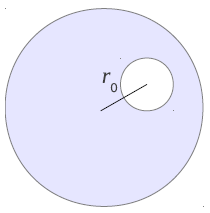
\includegraphics{Images/E2.png}
	\end{figure}
\end{frame}

\begin{frame}{Exercise 4}
Three infinitely large metal board carry charges $Q_1, Q_2, Q_3$ correspondingly 
and uniformly. What is the charge on each side of the three boards? 

\begin{figure}[H]
	\centering
	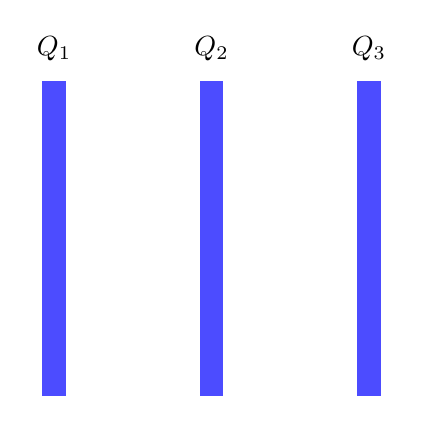
\begin{tikzpicture}
		\node[label=above:$Q_1$] (q1) at (0,4) {};
		\node[label=above:$Q_2$] (q2) at (2,4) {};
		\node[label=above:$Q_3$] (q3) at (4,4) {};
		\draw[line width=.3cm, blue!70] (0,0) -- (0,4);
		\draw[line width=.3cm, blue!70] (2,0) -- (2,4);
		\draw[line width=.3cm, blue!70] (4,0) -- (4,4);
	\end{tikzpicture}
\end{figure}
\end{frame}





\section{Appendix}

\begin{frame}
    \begin{center}
        \LARGE\bf Thank for listening!
    \end{center}
	
\end{frame}


\begin{frame}{\bf References}
	\nocite{*} % Display all references regardless of if they were cited
	\bibliography{rc1.bib}
	\bibliographystyle{plain}
\end{frame}

\end{document}

